\documentclass[11pt]{beamer}
\usetheme{Madrid}
\usepackage[utf8]{inputenc}
\usepackage[russian]{babel}
\usepackage{amsmath}
\usepackage{amsfonts}
\usepackage{amssymb}
\usepackage{here}
\usepackage{listings}
\beamertemplatenavigationsymbolsempty
\author[Косолапов С.А.]{Косолапов Семен Александрович}
\title[Современные проблемы ИиВТ]{Разработка макрорасширения для языка Kotlin. Обзор предметной области}
\date{\today} 
\institute[СПбПУ]{}
\begin{document}


\begin{frame}
\titlepage
\end{frame}


\begin{frame}
\frametitle{Что такое макросы и с чем их едят?}

\begin{itemize}
	\item Преобразователи исходного кода программ
	\item Используют специальный язык макрорасширений, элементы которого размещаются вместе с основной программой
\end{itemize}

\end{frame}

\begin{frame}
\frametitle{Как это работает?}

Макрорасширения являются средством метапрограммирования, то есть средством написания программ, порождающих другие программы

\begin{figure}[H]
	\begin{center}
		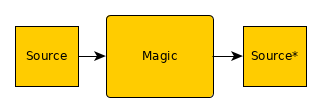
\includegraphics[scale=0.75]{pic/macro-work.png}
	\end{center}
\end{figure}

\end{frame}

\begin{frame}
\frametitle{Для чего они нужны?}

\begin{itemize}
	\item Исключение дублирования исходного кода
	\item Шаблонизация кода
	\item Создание удобных синтаксических конструкций
	\item Создание DSL
	\item Генерация built-in данных
	\item ...
\end{itemize}

\end{frame}

\begin{frame}
\frametitle{А почему для этого не использовать основной язык программирования?}

\begin{itemize}
	\item Это не всегда удобно программисту
	\item Может дольше выполняться (например, инлайнинг не всегда работает)
	\item А иногда это в принципе невозможно
\end{itemize}

\end{frame}

\begin{frame}
\frametitle{Как появились макрорасширения?}

\begin{itemize}
	\item Изначально -- в ассемблере для описания нескольких микроинструкций одной макроинструкцией
	\item К концу 50-х годов 20 века они приобрели тот вид, в котором используются сейчас
	\item Работают как простая текстовая подстановка
\end{itemize}

\end{frame}

\begin{frame}
\frametitle{А для языков высокого уровня?}

\begin{itemize}
	\item Первым был язык Lisp (1958 г.)
	\item Первый чисто функциональный язык программирования
	\item Программы как данные: гомоиконность
	\item Очень простой синтаксис, или отсутствие его как такового
	\item Удобен для экспериментов
	\item Первая реализация макросов -- в 1963 году
\end{itemize}

\end{frame}


\begin{frame}
\frametitle{Тогда что с императивными языками?}

\begin{itemize}
	\item Наиболее известный -- препроцессор языка C
	\item Просто текстовая подстановка
	\item Макросы очень широко используются в языке C
\end{itemize}

\end{frame}


\begin{frame}
\frametitle{Но там же столько проблем...}

\begin{itemize}
	\item Да, и эти проблемы могут сильно осложнить жизнь программисту
	\item Никакой проверки типов и даже <<целостности>> параметров
	\item Вызов макроса синтаксически выглядит так же, как и вызов функции
	\item Нет никакой обратной связи от основного языка к языку макрорасширения
\end{itemize}

\end{frame}


\begin{frame}
\frametitle{Больше скобочек!}

\begin{itemize}
\item плохой вариант
 
\#define discriminant(a, b, c) b*b - 4*a*c

\item хороший вариант

\#define discriminant(a, b, c) ((b)*(b) - 4*(a)*(c))
\end{itemize}

\end{frame}

\begin{frame}
\frametitle{Есть и другой выход - гигиена}

Переменные, объявленные внутри макроопределения, никогда не будут иметь конфликты с переменными, объявленными в области, где будет происходить раскрытие макро

\begin{itemize}
\item Впервые подход реализован для языка Scheme
\item Можем обезопасить код от непреднамеренного изменения значений переменных
\item Шаг к возможности определения рекурсивных макро
\item Есть различные подходы к реализации
\end{itemize}

\end{frame}

\begin{frame}
\frametitle{А если нужно внутри макроса обратиться к внешним объектам?}

\begin{itemize}
\item Для этого используется квазицитирование
\item При раскрытии макро должен знать, где находится, или хотя бы список объектов, к которым можно обратиться
\item Варианты использования неочевидны
\end{itemize}

\end{frame}

\begin{frame}
\frametitle{Macro-by-example}

\begin{itemize}
\item А что, если определять семантику аргументов вызова макро?
\item Pattern-matching
\item Для каждого варианта -- своя реализация
\item Сопоставлять можно количество аргументов и тип элемента AST
\item Регулярные выражения для повторений
\end{itemize}

\end{frame}


\begin{frame}
\frametitle{Macro-by-example: пример на Scheme}

(\textbf{declare-syntax} and

	\hspace*{20pt}[(and) true]
	
	\hspace*{20pt}[(and e) e]
	
	\hspace*{20pt}[(and e1 e2 ...) (if e1 (and e2 ...) false)])

\end{frame}


\begin{frame}[fragile]
\frametitle{Macro-by-example: пример на Rust}

\begin{lstlisting}
macro_rules! create_function {
    ($func_name:ident) => (
        fn $func_name() {
            println!("You called {:?}()", 
            		stringify!($func_name))
        }
    )
}

create_function!(foo); // -> You called "foo"()
create_function!(bar); // -> You called "bar"()

\end{lstlisting}

\end{frame}


\begin{frame}[fragile]
\frametitle{Macro-by-example: пример на Rust}

\begin{lstlisting}

macro_rules! find_min {
    ($x:expr) => ($x);
    ($x:expr, $($y:expr),+) => (
        std::cmp::min($x, find_min!($($y),+))
    )
}

fn main() {
    println!("{}", find_min!(1u32));
    // -> 1
    println!("{}", find_min!(1u32 + 2 , 2u32)); 
    // -> 2
    println!("{}", find_min!(5u32, 2u32 * 3, 4u32)); 
    // -> 4
}

\end{lstlisting}

\end{frame}


\begin{frame}
\frametitle{Что требуется?}

Разработать препроцессор макроопределений, расширяющих язык Kotlin.

\begin{itemize}
	\item На входе - программа на расширенном языке Kotlin с конструкциями, позволяющими определять и применять макро
	\item На выходе - программа на <<чистом>> языке Kotlin
\end{itemize}

\end{frame}


\begin{frame}
\frametitle{Используемые принципы}

\begin{itemize}
	\item Macro-by-example
	\item Hygienic macros
\end{itemize}

\end{frame}


\begin{frame}
\frametitle{Как это сделать?}

\begin{itemize}
	\item Использование кода компилятора языка Kotlin
	\item Основная проблема в том, что внутри AST макроса будет AST исходной программы
	\item ...Если что-то пойдёт не так, то придётся определять синтаксис с нуля
\end{itemize}

\end{frame}

\begin{frame}[fragile]
\frametitle{Что должно получиться?}

\begin{lstlisting}

macro define_hello_world {
    (function:ident) -> {
            fun $function() {
                println("Hello, world!")
            }
    }
}

fun someFun() {
    define_hello_world!(hw_in_fun)
    hw_in_fun() // -> "Hello, world!"
}

\end{lstlisting}

\end{frame}

\begin{frame}
\huge{\centerline{Спасибо за внимание!}}
\end{frame}


\end{document}
